\chapter{需求分析}\label{chap:feasibility}
\thispagestyle{empty}
\section{功能需求}
% 本平台的用户可以分为三类:分析团队、调度员和管理者。

对于分析团队,他们对该平台有以下需求:
\begin{enumerate}
    \item 由平台生成查看单车分布图,对应图\ref{GenerateBikeDistributionMap}中的用例\texttt{Generate Bike Distribution Map};
    \item 由平台生成调度日志,对应图\ref{ProduceBikeSchedulingLog}中的用例\texttt{Produce Bike Scheduling Log};
    \item 由平台生成单车使用情况的空间分布,对应图\ref{GenerateBikeUsageMap}中的用例\texttt{Generate Bike Usage Map}。
    \item 由平台生成单车状况统计信息,对应图\ref{ProduceBikeStatusStatistics}中的用例\texttt{Produce Bike Status Statistics}。
\end{enumerate}

对于调度员,他们对于该平台有以下需求:
\begin{enumerate}
    \item 调度员可以在平台中上传调度信息,对应图\ref{UploadSchedulingLog}中的用例\texttt{Upload Scheduling Log};
    \item 调度员可以在平台中更新单车状态信息,对应图\ref{UpdateSingleBikeStatus}中的用例\texttt{Update Single Bike Status}。
\end{enumerate}

对于管理者,在分析团队的需求基础之上,他们对于该平台有还以下需求:
\begin{enumerate}
    \item 管理者可以通过平台添加或删除单车信息,对应图\ref{ModifyBikeList}中的用例\texttt{Modify Bike List};
    \item 管理者可以通过平台添加或删除停车区域信息,对应图\ref{ModifyParkingAreaList}中的用例\texttt{Modify Parking Area List}。
    \item 通过平台全局更新单车状态,对应图\ref{UpdateBikeStatusGlobally}中的用例\texttt{Update Bike Status Globally}。
\end{enumerate}

处于安全性考虑,平台还需要对上述三类用户进行分级。

同时,该平台需要处理由共享单车在开关锁时上传的信息,对应图\ref{UpdateBikeInformation}中的用例\texttt{Update Bike Info}。

整个系统的用例汇总如图\ref{UseCase}所示。

\begin{figure}[!htbp]
    \centering
    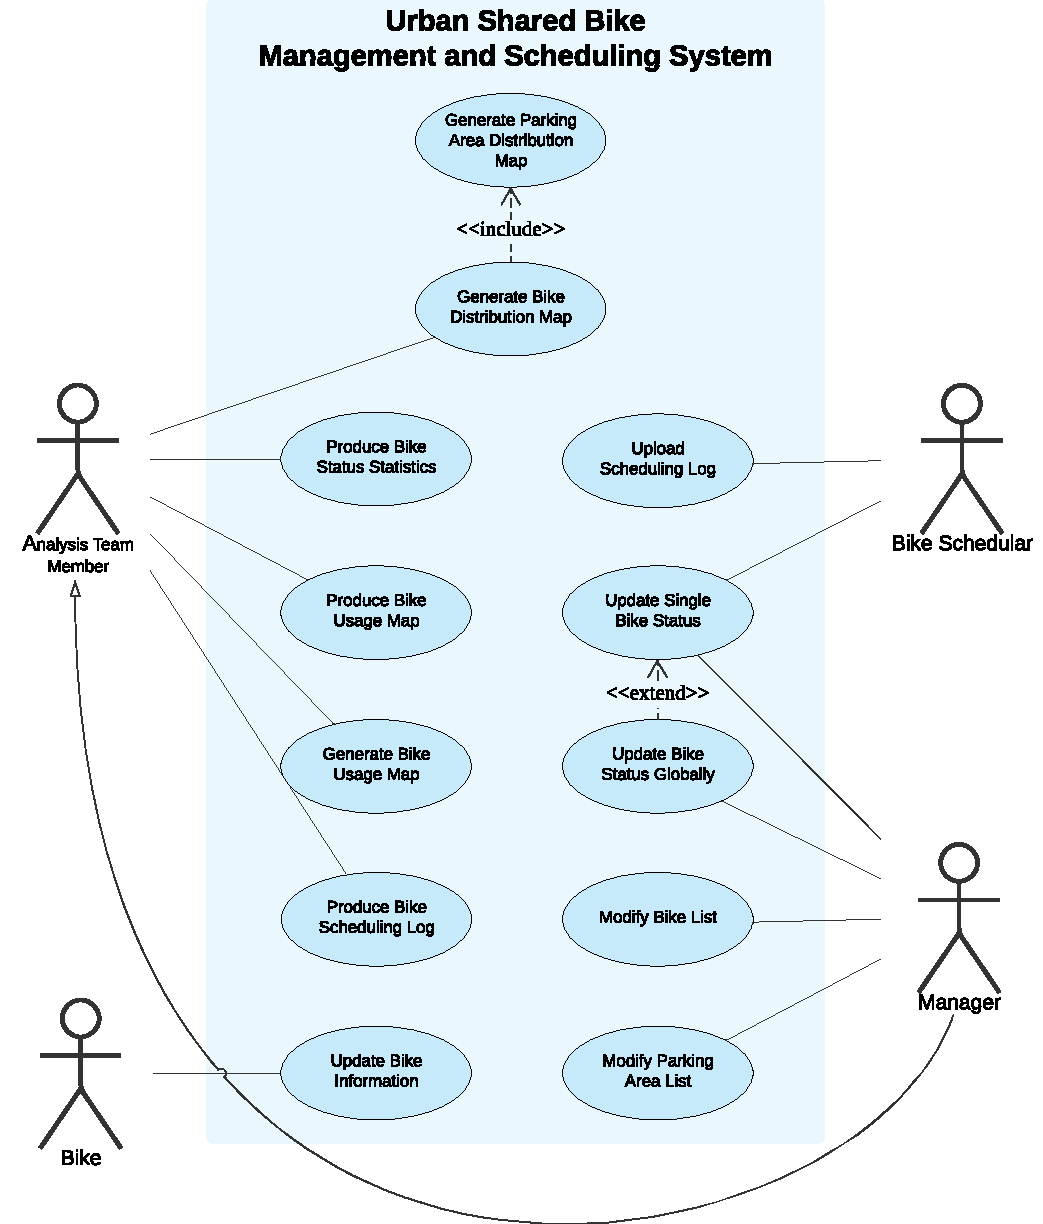
\includegraphics[width=0.99\textwidth]{figures/UseCase.pdf}
    \caption{用例汇总}\label{UseCase}
\end{figure}


\begin{figure}
    \centering
 \begin{mdframed}[leftmargin=0pt, rightmargin=0pt]
    \textbf{简要说明}

    用例\texttt{Generate Bike Distribution Map}使得分析团队成员和调度员能够查看共享单车的实时分布。

\noindent\rule{\textwidth}{0.5pt} % 实线分割线
    \textbf{分步说明}

    \begin{enumerate}
        \item 系统从数据库中收集所有共享单车的坐标及其状态;
        \item 系统依据单车坐标将单车标注在电子地图中;
        \item 系统依据单车坐标生成热力图;
        \item 系统通过用例\texttt{Generate Parking Area Distribution Map}在地图中标注停车区域;
        \item 系统调整地图窗口显示区域。
    \end{enumerate}
\end{mdframed}   
\caption{用例\texttt{Generate Bike Distribution Map}}\label{GenerateBikeDistributionMap}
\end{figure}

\begin{figure}
    \centering
 \begin{mdframed}[leftmargin=0pt, rightmargin=0pt]
    \textbf{简要说明}

    用例\texttt{Generate Parking Area Distribution Map}使得分析团队成员和调度员能够查看停车区域的分布情况。

\noindent\rule{\textwidth}{0.5pt} % 实线分割线
    \textbf{分步说明}

    \begin{enumerate}
        \item 系统从数据库中收集所有停车区域的中心坐标与半径;
        \item 系统利用中心坐标与半径在地图中绘制圆形区域以表示停车区域;
    \end{enumerate}
\end{mdframed}   
\caption{用例\texttt{Generate Parking Area Distribution Map}}\label{GenerateParkingAreaDistributionMap}
\end{figure}

\begin{figure}
    \centering
 \begin{mdframed}[leftmargin=0pt, rightmargin=0pt]
    \textbf{简要说明}

    用例\texttt{Upload Scheduling Log}使得调度员能够上传调度日志。

\noindent\rule{\textwidth}{0.5pt} % 实线分割线
    \textbf{分步说明}

    \begin{enumerate}
        \item 调度员通过API接口向系统上传调度日志;
        \item 系统将数据保存至\texttt{scheduling}表中;
    \end{enumerate}
\end{mdframed}   
\caption{用例\texttt{Upload Scheduling Log}}\label{UploadSchedulingLog}
\end{figure}



\begin{figure}
    \centering
 \begin{mdframed}[leftmargin=0pt, rightmargin=0pt]
    \textbf{简要说明}

    用例\texttt{Update Single Bike Status}使得调度员能够更新单个单车的状态。

\noindent\rule{\textwidth}{0.5pt} % 实线分割线
    \textbf{分步说明}

    \begin{enumerate}
        \item 调度员通过API接口向系统上传修改表单;
        \item 系统将修改表单保存至\texttt{to\_be\_reviewed\_status},\texttt{to\_be\_reviewed\_proof\_material}和\texttt{to\_be\_reviewed}中;
        \item 管理者审核表单;
        \item 若通过,则系统更新\texttt{bike\_status};否则,系统不对数据进行更新。
        \item 系统从\texttt{to\_be\_reviewed},\texttt{to\_be\_reviewed\_status}和\texttt{to\_be\_reviewed\_proof\_material}中删除相关数据;
    \end{enumerate}
\end{mdframed}   
\caption{用例\texttt{Update Single Bike Status}}\label{UpdateSingleBikeStatus}
\end{figure}

\begin{figure}
    \centering
 \begin{mdframed}[leftmargin=0pt, rightmargin=0pt]
    \textbf{简要说明}

    用例\texttt{Produce Bike Scheduling Log}使得分析团队成员能够获取单车的调度日志。

\noindent\rule{\textwidth}{0.5pt} % 实线分割线
    \textbf{分步说明}

    \begin{enumerate}
        \item 分析团队成员输入待查询单车的id号;
        \item 系统在\texttt{scheduling}表中查询与指定单车相关的调度信息;
        \item 系统按照时间顺序将调度信息进行整理,并利用\texttt{action}域进行配对;
        \item 系统打印整理后的调度信息。
    \end{enumerate}
\end{mdframed}   
\caption{用例\texttt{Produce Bike Scheduling Log}}\label{ProduceBikeSchedulingLog}
\end{figure}

\begin{figure}
    \centering
 \begin{mdframed}[leftmargin=0pt, rightmargin=0pt]
    \textbf{简要说明}

    用例\texttt{Generate Bike Usage Map}使得分析团队成员能够获取单车的使用情况时空分布。

\noindent\rule{\textwidth}{0.5pt} % 实线分割线
    \textbf{分步说明}

    \begin{enumerate}
        \item 分析团队成员选择查询时间段;
        \item 系统在\texttt{usage}表中查询所有单车在指定时间段内的使用情况;
        \item 系统将筛选得到的使用情况按照时间顺序进行整理,并利用\texttt{action}域进行配对;
        \item 系统将使用情况标记在电子地图中。
    \end{enumerate}
\end{mdframed}   
\caption{用例\texttt{Generate Bike Usage Map}}\label{GenerateBikeUsageMap}
\end{figure}

\begin{figure}
    \centering
 \begin{mdframed}[leftmargin=0pt, rightmargin=0pt]
    \textbf{简要说明}

    用例\texttt{Produce Bike Status Statistics}使得分析团队成员能够获取单车的状态统计信息。

\noindent\rule{\textwidth}{0.5pt} % 实线分割线
    \textbf{分步说明}

    \begin{enumerate}
        \item 系统通过\texttt{bike\_status}表统计处于各状态的单车比例;
        \item 系统打印状态统计信息。
    \end{enumerate}
\end{mdframed}   
\caption{用例\texttt{Produce Bike Status Statistics}}\label{ProduceBikeStatusStatistics}
\end{figure}

\begin{figure}
    \centering
 \begin{mdframed}[leftmargin=0pt, rightmargin=0pt]
    \textbf{简要说明}

    用例\texttt{Update Bike Information}使得单车能够上传当前车辆信息。

\noindent\rule{\textwidth}{0.5pt} % 实线分割线
    \textbf{分步说明}

    \begin{enumerate}
        \item 单车通过API接口向系统上传位置、电池电量信息以及触发动作(开锁或关锁);
        \item 系统根据数据更新\texttt{bike}表;
        \item 系统根据\texttt{parking\_area}中的数据来判断是否需要更新单车状态。
    \end{enumerate}
\end{mdframed}   
\caption{用例\texttt{Update Bike Information}}\label{UpdateBikeInformation}
\end{figure}

\begin{figure}
    \centering
 \begin{mdframed}[leftmargin=0pt, rightmargin=0pt]
    \textbf{简要说明}

    用例\texttt{Update Bike Status Globally}使得管理者能够批量更新单车状态。

\noindent\rule{\textwidth}{0.5pt} % 实线分割线
    \textbf{分步说明}

    \begin{enumerate}
        \item 管理者在系统中确定状态更新的条件;
        \item 如果更新“低电量”状态,则系统根据\texttt{bike}表中的\texttt{battery\_remaining\_capacity}进行更新;
        \item 如果更新“闲置”状态,则系统根据\texttt{usage}表中的数据来获取各单车最近的关锁时间,依据此进行更新;
        \item 如果更新“长期未关锁”状态,则系统根据\texttt{usage}表中的数据来获取各单车最近的没有对应关锁行动的开锁行动,依据此进行更新;
        \item 如果更新“型号老旧”状态,则系统根据\texttt{bike}中的\texttt{production\_date}域来进行更新。
    \end{enumerate}
\end{mdframed}   
\caption{用例\texttt{Update Bike Status Globally}}\label{UpdateBikeStatusGlobally}
\end{figure}

\begin{figure}
    \centering
 \begin{mdframed}[leftmargin=0pt, rightmargin=0pt]
    \textbf{简要说明}

    用例\texttt{Modify Bike List}使得管理者能够添加或删除单车信息。

\noindent\rule{\textwidth}{0.5pt} % 实线分割线
    \textbf{分步说明}

    \begin{enumerate}
        \item 若管理者要求添加单车信息,则:
        \begin{enumerate}
            \item 管理者填写单车信息;
            \item 系统向\texttt{bike}表中插入该信息;
            \item 系统更新\texttt{contain}表。
        \end{enumerate}
        \item 若管理者要求删除单车信息,则:
        \begin{enumerate}
            \item 管理者输入待删除单车id;
            \item 系统在数据库中删除指定单车的相关信息。
        \end{enumerate}
    \end{enumerate}
\end{mdframed}   
\caption{用例\texttt{Modify Bike List}}\label{ModifyBikeList}
\end{figure}

\begin{figure}
    \centering
 \begin{mdframed}[leftmargin=0pt, rightmargin=0pt]
    \textbf{简要说明}

    用例\texttt{Modify Parking Area List}使得管理者能够添加或删除停车区域信息。

\noindent\rule{\textwidth}{0.5pt} % 实线分割线
    \textbf{分步说明}

    \begin{enumerate}
        \item 若管理者要求添加停车区域信息,则:
        \begin{enumerate}
            \item 管理者填写停车区域信息;
            \item 系统向\texttt{parking\_area}表中插入该信息;
            \item 系统更新\texttt{contain}表。
        \end{enumerate}
        \item 若管理者要求删除停车区域信息,则:
        \begin{enumerate}
            \item 管理者输入待删除停车区域id;
            \item 系统在数据库中删除指定停车区域的相关信息。
        \end{enumerate}
    \end{enumerate}
\end{mdframed}   
\caption{用例\texttt{Modify Parking Area List}}\label{ModifyParkingAreaList}
\end{figure}

\section{数据字典}
数据字典如表\ref{DataDictionary1}-\ref{DataDictionary3}所示。
\begin{table}
\centering
\caption{数据字典(调度相关部分)}
\label{DataDictionary1}
\begin{tabular}{lll}\toprule
  数据元素名称&描述&备注\\\midrule
scheduling log            &
   \makecell[l]{
    该数据元素包含以下域:\\
    \quad 坐标\\
    \quad 时间\\
    \quad 动作\\
    }                &\makecell[l]{坐标由经纬度构成;\\动作为“开始”或“结束”}              \\
scheduling history&与scheduling log包含相同的域&数据库中存储的所有调度记录\\
required scheduling history&与scheduling log包含相同的域&指定单车的历史调度记录\\
 \bottomrule
\end{tabular}
\end{table}

\begin{table}
\centering
\caption{数据字典(停车区域相关部分)}
\label{DataDictionary2}
\begin{tabular}{lll}\toprule
  数据元素名称&描述&备注\\\midrule
parking area info          &   \makecell[l]{
    该数据元素包含以下域:\\
    \quad 停车区域名称\\
    \quad 停车区域坐标\\
    \quad 停车区域半径\\
    }                &\makecell[l]{坐标由经纬度构成;\\半径单位为米}             \\
 \bottomrule
\end{tabular}
\end{table}

\begin{table}
\centering
\caption{数据字典(审核相关部分)}
\label{DataDictionary3}
\begin{tabular}{lll}\toprule
  数据元素名称&描述&备注\\\midrule
change form                         &  \makecell[l]{
    该数据元素包含以下域:\\
    \quad 单车id\\
    \quad 更新后的单车状态\\
    \quad 证明材料\\
    }&\makecell[l]{证明材料为图片}    \\
comment                    &0或1             &  \makecell[l]{为1代表通过,\\否则拒绝单车状态更改生效}    \\
Review                     &\makecell[l]{输入参数:\\\quad 待改变状态\\\quad 支撑材料\\输出参数:\\\quad 审核意见}&\makecell[l]{
    该流程的步骤为:\\
    \quad 管理者查看待更改状态和相应的图片\\
    \quad 管理者作出审核意见\\
    }          \\
 \bottomrule
\end{tabular}
\end{table}
\begin{longtable}{lll}
    \caption{数据字典(单车相关部分)}\label{DataDictionary4} \\
    \toprule
  数据元素名称&描述&备注\\
  \midrule
  \endfirsthead
    \toprule
  数据元素名称&描述&备注\\
  \midrule
  \endhead

  \midrule
\multicolumn{3}{r}{表格继续下一页} \\
\bottomrule
\endfoot

% 设置表格最后一页的表尾内容
\bottomrule
\endlastfoot

bike status       &    \makecell[l]{
    取值范围如下:\\
    \quad 正常\\
    \quad 违规停放\\
    \quad 低电量\\
    \quad 闲置\\
    \quad 长期未关锁\\
    \quad 异常\\
    \quad 待维修\\
    \quad 型号老旧\\
    \quad 入库\\
    }         &\makecell[l]{ 描述单车当前状态,\\可由多个状态合理组合而成 }\\
updated bike status               & 与bike status一致                 &描述更新后的单车状态    \\
bike info                         &  \makecell[l]{
    该数据元素包含以下域:\\
    \quad 单车id\\
    \quad 单车坐标\\
    \quad 单车生产日期\\
    }&\makecell[l]{用于初始化单车数据\\单车生产日期格式为YYYY:MM:DD}    \\
uploaded data                         &  \makecell[l]{
    该数据元素包含以下域:\\
    \quad 单车id\\
    \quad 单车坐标\\
    \quad 单车剩余电量\\
    \quad 行动\\
    }&\makecell[l]{由单车上传的信息\\行动为1代表是开锁动作,\\为0代表是关锁动作 }    \\
previous status                         &  \makecell[l]{
    该数据元素包含以下域:\\
    \quad 单车状态\\
    \quad 最近使用时间\\
    }&用于和待更新状态进行对比 \\
map data                         &  \makecell[l]{
    该数据元素包含以下域:\\
    \quad 单车id\\
    \quad 单车状态\\
    \quad 单车坐标\\
    }&用于绘制单车分布图 \\
usage data                         &  \makecell[l]{
    该数据元素包含以下域:\\
    \quad 单车id\\
    \quad 起始坐标\\
    \quad 起始时间\\
    \quad 结束坐标\\
    \quad 结束时间\\
    }&用于绘制单车使用情况时空图 \\
uploaded usage data                         &  \makecell[l]{
    该数据元素包含以下域:\\
    \quad 单车id\\
    \quad 单车坐标\\
    \quad 行动时间\\
    \quad 行动\\
    }&\makecell[l]{由单车上传的信息\\行动为1代表是开锁动作,\\为0代表是关锁动作 } \\
bike status statistics     &处于各状态的单车数量占总数的比例          &  格式为**.**\%            \\
time period                &指定时间段          &  用于生成单车使用情况分布图            \\
uploaded bike info                         &  \makecell[l]{
    该数据元素包含以下域:\\
    \quad 单车坐标\\
    \quad 剩余电量\\
    \quad 状态更新\\
    }&\makecell[l]{依据单车坐标和剩余电量更新状态 } \\

\end{longtable}


\section{数据流图}
数据流图如图\ref{DataFlow}所示。

除过程Review外,数据流图中的其余过程已在图\ref{GenerateBikeDistributionMap}-\ref{ModifyParkingAreaList}中以用例的形式来描述,所以不在数据字典中重复,
其中流程Update Bike Status对应于用例\texttt{Update Bike Status Globally}和\texttt{Update Single Bike Status}外,其余流程都对应于其同名用例。

\begin{figure}[!htbp]
    \centering
    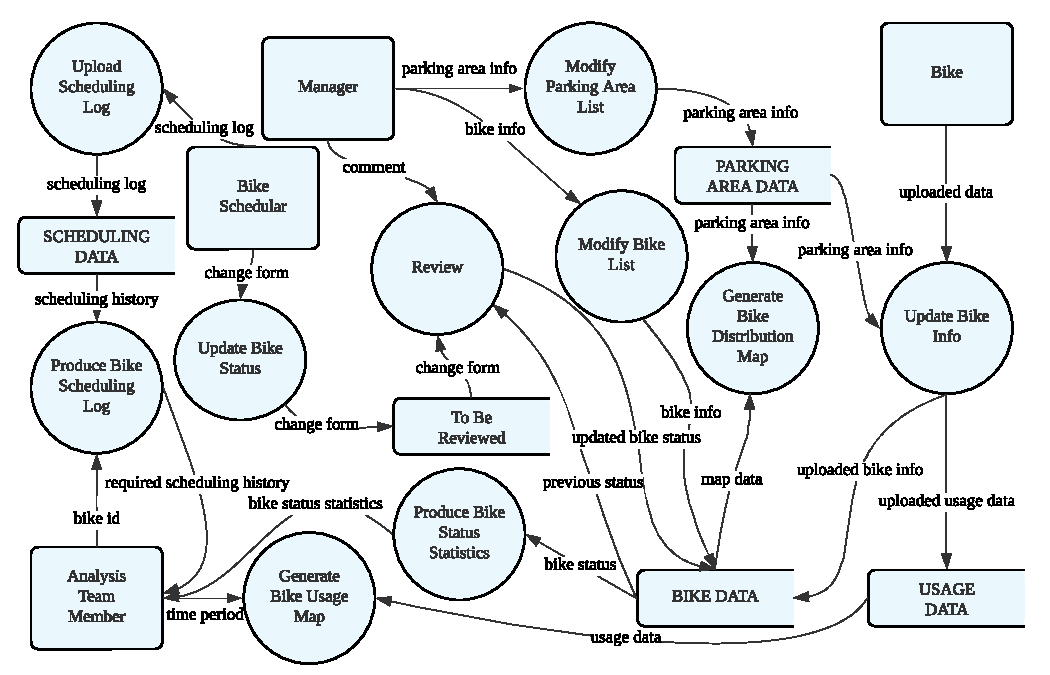
\includegraphics[width=\textwidth]{figures/DataFlow.pdf}
    \caption{数据流图}\label{DataFlow}
\end{figure}
